\documentclass{beamer}
\usepackage[utf8]{inputenc}

\usetheme{Madrid}
\usecolortheme{default}
\usepackage{amsmath,amssymb,amsfonts,amsthm}
\usepackage{txfonts}
\usepackage{tkz-euclide}
\usepackage{listings}
\usepackage{adjustbox}
\usepackage{array}
\usepackage{tabularx}
\usepackage{gvv}
\usepackage{lmodern}
\usepackage{circuitikz}
\usepackage{tikz}
\usepackage{graphicx}

\setbeamertemplate{page number in head/foot}[totalframenumber]

\usepackage{tcolorbox}
\tcbuselibrary{minted,breakable,xparse,skins}



\definecolor{bg}{gray}{0.95}
\DeclareTCBListing{mintedbox}{O{}m!O{}}{%
  breakable=true,
  listing engine=minted,
  listing only,
  minted language=#2,
  minted style=default,
  minted options={%
    linenos,
    gobble=0,
    breaklines=true,
    breakafter=,,
    fontsize=\small,
    numbersep=8pt,
    #1},
  boxsep=0pt,
  left skip=0pt,
  right skip=0pt,
  left=25pt,
  right=0pt,
  top=3pt,
  bottom=3pt,
  arc=5pt,
  leftrule=0pt,
  rightrule=0pt,
  bottomrule=2pt,
  toprule=2pt,
  colback=bg,
  colframe=orange!70,
  enhanced,
  overlay={%
    \begin{tcbclipinterior}
    \fill[orange!20!white] (frame.south west) rectangle ([xshift=20pt]frame.north west);
    \end{tcbclipinterior}},
  #3,
}
\lstset{
    language=C,
    basicstyle=\ttfamily\small,
    keywordstyle=\color{blue},
    stringstyle=\color{orange},
    commentstyle=\color{green!60!black},
    numbers=left,
    numberstyle=\tiny\color{gray},
    breaklines=true,
    showstringspaces=false,
}
\begin{document}

\title 
{9.4.18}
\date{Oct 5,2025}


\author 
{ADUDOTLA SRIVIDYA -EE25BTECH11006}






\frame{\titlepage}

\begin{frame}{Question}
\textbf{Question}: \\
Find the roots of the quadratic equation graphically.
\begin{align}
4x^2 + 4\sqrt{3}x + 3 = 0
\end{align}
\end{frame}

\begin{frame}{Solution}
\begin{align}
y = 4x^2 + 4\sqrt{3}x + 3 = 0
\end{align}

This equation can be represented as the conic
\begin{align}
\vec{x^T}\vec{V}\vec{x} + 2\vec{u^T}\vec{x} + f = 0
\end{align}
\begin{align}
\vec{V} = \myvec{4 & 0 \\ 0 & 0}, \vec{u} = \myvec{2\sqrt{3} \\ 0}, f = 3
\end{align}
\end{frame}

\begin{frame}{Solution}
To find the roots, we find the points of intersection of the conic with the x-axis.
\begin{align}
\vec{x} = \vec{h} + k_i\vec{m}    
\end{align}
\begin{align}
\vec{h}=\myvec{0 \\ 0}, \vec{m} = \myvec{1 \\ 0}
\end{align}
\end{frame}

\begin{frame}{Solution}
The value of $k_i$ can be found out by solving the line and conic equation
\begin{align}
(\vec{h} + k_i \vec{m})^{\top} \vec{V} (\vec{h} + k_i \vec{m}) + 2\vec{u}^{\top} (\vec{h} + k_i \vec{m}) + f &= 0 \\
\implies k_i^{2} \vec{m}^{\top}\vec{V}\vec{m} + 2k_i \vec{m}^{\top} (\vec{V}\vec{h} + \vec{u}) + \vec{h}^{\top}\vec{V}\vec{h} + 2\vec{u}^{\top}\vec{h} + f &= 0 \\
\text{or, } k_i^{2} \vec{m}^{\top}\vec{V}\vec{m} + 2k_i \vec{m}^{\top} (\vec{V}\vec{h} + \vec{u}) + g(\vec{h}) &= 0
\end{align}
\end{frame}

\begin{frame}{Solution}
Solving the above quadratic gives the equation
\begin{align}
k_i = \frac{1}{\vec{m}^{\top}\vec{V}\vec{m}}
\brak{
    -\vec{m}^{\top} (\vec{V}\vec{h} + \vec{u})
    \;\pm\;
    \sqrt{ \sbrak{\vec{m}^{\top}(\vec{V}\vec{h} + \vec{u})}^2
    - g(\vec{h}) \, (\vec{m}^{\top}\vec{V}\vec{m}) }
    }
\end{align}

\begin{align}
\therefore k_i = \frac{-2\sqrt{3}}{4} = \frac{-\sqrt{3}}{2}
\end{align}
\end{frame}

\begin{frame}{Solution}
\begin{align}
\implies k_1 = k_2 = \frac{-\sqrt{3}}{2}
\end{align}

\begin{align}
\therefore \vec{x} = \vec{h} + k_i\vec{m} = \myvec{-\frac{\sqrt{3}}{2} \\ 0}
\end{align}
\end{frame}

\begin{frame}[fragile]
\frametitle{Python,C,Python+C codes}
codes permalink
\end{frame}

\begin{frame}{Plot}
\begin{figure}[h!]
    \centering
    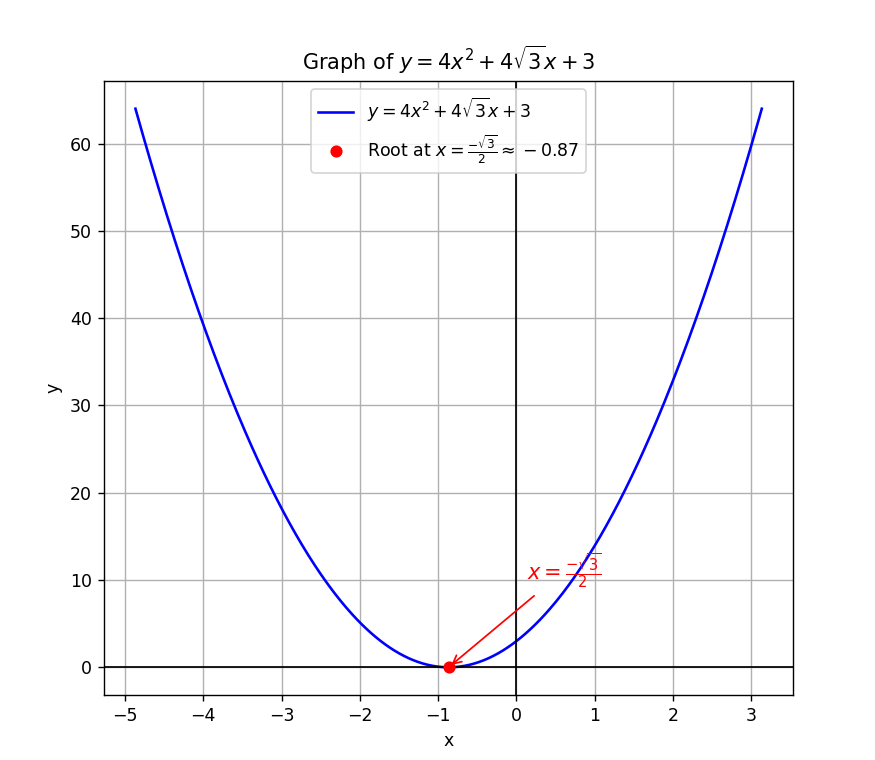
\includegraphics[height=0.5\textheight, keepaspectratio]{figs/fig.png}
    \label{figure_9_4_18}
\end{figure}
\end{frame}

\end{document}
